% 2 Theorie

% alt
% Auch in neueren Schriften der Extremismustheoretiker*innen bleibt die Definition \emph{ex negativo} primäres Abgrenzungskriterium; so heißt es schon im ersten Satz der Einleitung eines von Hirscher und Jesse herausgegebenen Sammelbandes: „Extremismus ist das Gegenstück zum demokratischen Verfassungsstaat`` \autocite*[9]{hirscherExtremismusDeutschland2013}. Es sind jedoch auch eine Reihe positiver Definitionsmerkmale gefunden worden, die anschließend genannt werden; darunter „Freund-Feind-Stereotype``, „ideologischer Dogmatismus``, „Missionierungsbewusstsein``, „der Glaube an ein erkennbares und vorgegebenes Gemeinwohl und historische Gesetzmäßigkeiten``, „Illegitimität unterschiedlicher Meinungen und Interessen``, „Verschwörungstheorien`` sowie die „Rechtfertigung von Gewalt`` \autocite[9-10]{hirscherExtremismusDeutschland2013}. Während die Ablehnung der FdGO definitorischer Kern bleibt, werden mehrere der genannten Elemente der Definition \emph{ex positivo} durch Modifikatoren wie „in der Regel``, „kaum``, „meist`` und „zuweilen`` in ihrer Geltung eingeschränkt. Die genannten Merkmale gelten dabei für jede Form von Extremismus und sollen ihn eindeutig zur gemäßigten, demokratischen Mitte der Gesellschaft abgrenzen. Die Extreme sind dabei in den Anfängen der Extremismustheorie, die sich noch auf den Bereich des politischen Extremismus beschränkte, als Pole des politischen Spektrums auf der Rechts-Links-Achse zu verstehen. Einer der Kerngedanken lautet jedoch, dass sich die beiden Enden des Spektrums zwar in ihren inhaltlichen Zielen unterscheiden, jedoch zugleich mit der Ablehnung der FdGO eine bedeutende Eigenschaft teilen. Diese Nähe der entgegengesetzten Extreme begründet sodann die bekannte Darstellung des politischen Extremismus als Hufeisen (\figref{fig:hufeisen}). Dazu konstatiert Backes:
%
% \begin{quote}
% Um die Vermischung gegenläufiger Traditionslinien zu vermeiden, koppelt man die Begriffe „links`` und „rechts`` häufig an das Gegensatzpaar „extremistisch`` und „gemäßigt``, wobei „Mäßigung`` im Sinne des demokratischen Verfassungsstaates verstanden wird. Das politische Spektrum läßt sich dann in der Form eines Hufeisens darstellen, dessen Pole einander entfernt und benachbart zugleich sind. Das Hufeisen-Modell {[}\ldots{]} trägt der Tatsache Rechnung, daß die Grenzlinie zwischen politischem Extremismus und demokratischem Verfassungsstaat für die Bewertung politischer Phänomene von größerer Bedeutung ist als die jeweilige Stellung auf der Rechts-Links-Achse. \autocite[251]{backesPolitischerExtremismusDemokratischen1989}
% \end{quote}
%
% \begin{figure}
%   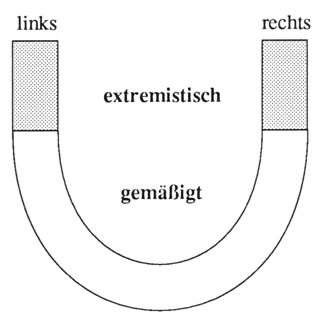
\includegraphics[width=.5\textwidth]{figures/media/image6.jpeg}
%   \caption{\label{fig:hufeisen}Das Hufeisen-Modell der Extremismustheorie (Schaubild 7 aus \citealt[252]{backesPolitischerExtremismusDemokratischen1989}).}
% \end{figure}

%  neu 

% Auch in neueren Schriften der Extremismustheoretiker*innen bleibt die Definition \emph{ex negativo} primäres Abgrenzungskriterium; so heißt es schon im ersten Satz der Einleitung eines von Hirscher und Jesse herausgegebenen Sammelbandes: „Extremismus ist das Gegenstück zum demokratischen Verfassungsstaat`` \autocite*[9]{hirscherExtremismusDeutschland2013}. Es sind jedoch auch eine Reihe positiver Definitionsmerkmale gefunden worden, die anschließend genannt werden; darunter „Freund-Feind-Stereotype``, „ideologischer Dogmatismus``, „Missionierungsbewusstsein``, „der Glaube an ein erkennbares und vorgegebenes Gemeinwohl und historische Gesetzmäßigkeiten``, „Illegitimität unterschiedlicher Meinungen und Interessen``, „Verschwörungstheorien`` sowie die „Rechtfertigung von Gewalt`` \autocite[9-10]{hirscherExtremismusDeutschland2013}. Während die Ablehnung der FdGO definitorischer Kern bleibt, werden mehrere der genannten Elemente der Definition \emph{ex positivo} durch Modifikatoren wie „in der Regel``, „kaum``, „meist`` und „zuweilen`` in ihrer Geltung eingeschränkt. Die genannten Merkmale gelten dabei für jede Form von Extremismus und sollen ihn eindeutig zur gemäßigten, demokratischen Mitte der Gesellschaft abgrenzen. Die Extreme sind dabei in den Anfängen der Extremismustheorie, die sich noch auf den Bereich des politischen Extremismus beschränkte, als Pole des politischen Spektrums auf der Rechts-Links-Achse zu verstehen. Einer der Kerngedanken lautet jedoch, dass sich die beiden Enden des Spektrums zwar in ihren inhaltlichen Zielen unterscheiden, jedoch zugleich mit der Ablehnung der FdGO eine bedeutende Eigenschaft teilen. Diese Nähe der entgegengesetzten Extreme begründet sodann die bekannte Darstellung des politischen Extremismus als Hufeisen (siehe bereits Schaubild 7 in \citealt[252]{backesPolitischerExtremismusDemokratischen1989}). Dazu konstatiert Backes:
%
% \begin{quote}
% Um die Vermischung gegenläufiger Traditionslinien zu vermeiden, koppelt man die Begriffe „links`` und „rechts`` häufig an das Gegensatzpaar „extremistisch`` und „gemäßigt``, wobei „Mäßigung`` im Sinne des demokratischen Verfassungsstaates verstanden wird. Das politische Spektrum läßt sich dann in der Form eines Hufeisens darstellen, dessen Pole einander entfernt und benachbart zugleich sind. Das Hufeisen-Modell {[}\ldots{]} trägt der Tatsache Rechnung, daß die Grenzlinie zwischen politischem Extremismus und demokratischem Verfassungsstaat für die Bewertung politischer Phänomene von größerer Bedeutung ist als die jeweilige Stellung auf der Rechts-Links-Achse. \autocite[251]{backesPolitischerExtremismusDemokratischen1989}
% \end{quote}








% alt

% 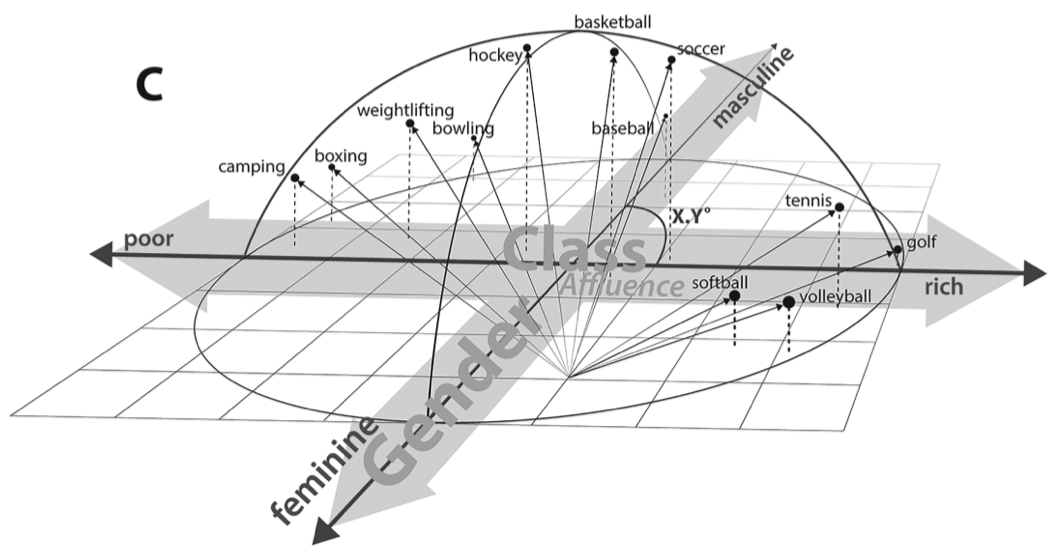
\includegraphics[width=\textwidth]{figures/media/image8.png}
%   \caption{\label{fig:kozlowski}Semantische Projektion der Wortvektoren unterschiedlicher Sportarten auf zwei ‚kulturelle Dimensionen` (\emph{Figure} 2c aus \citealt[913]{kozlowskiGeometryCultureAnalyzing2019}).}
% % neu

% 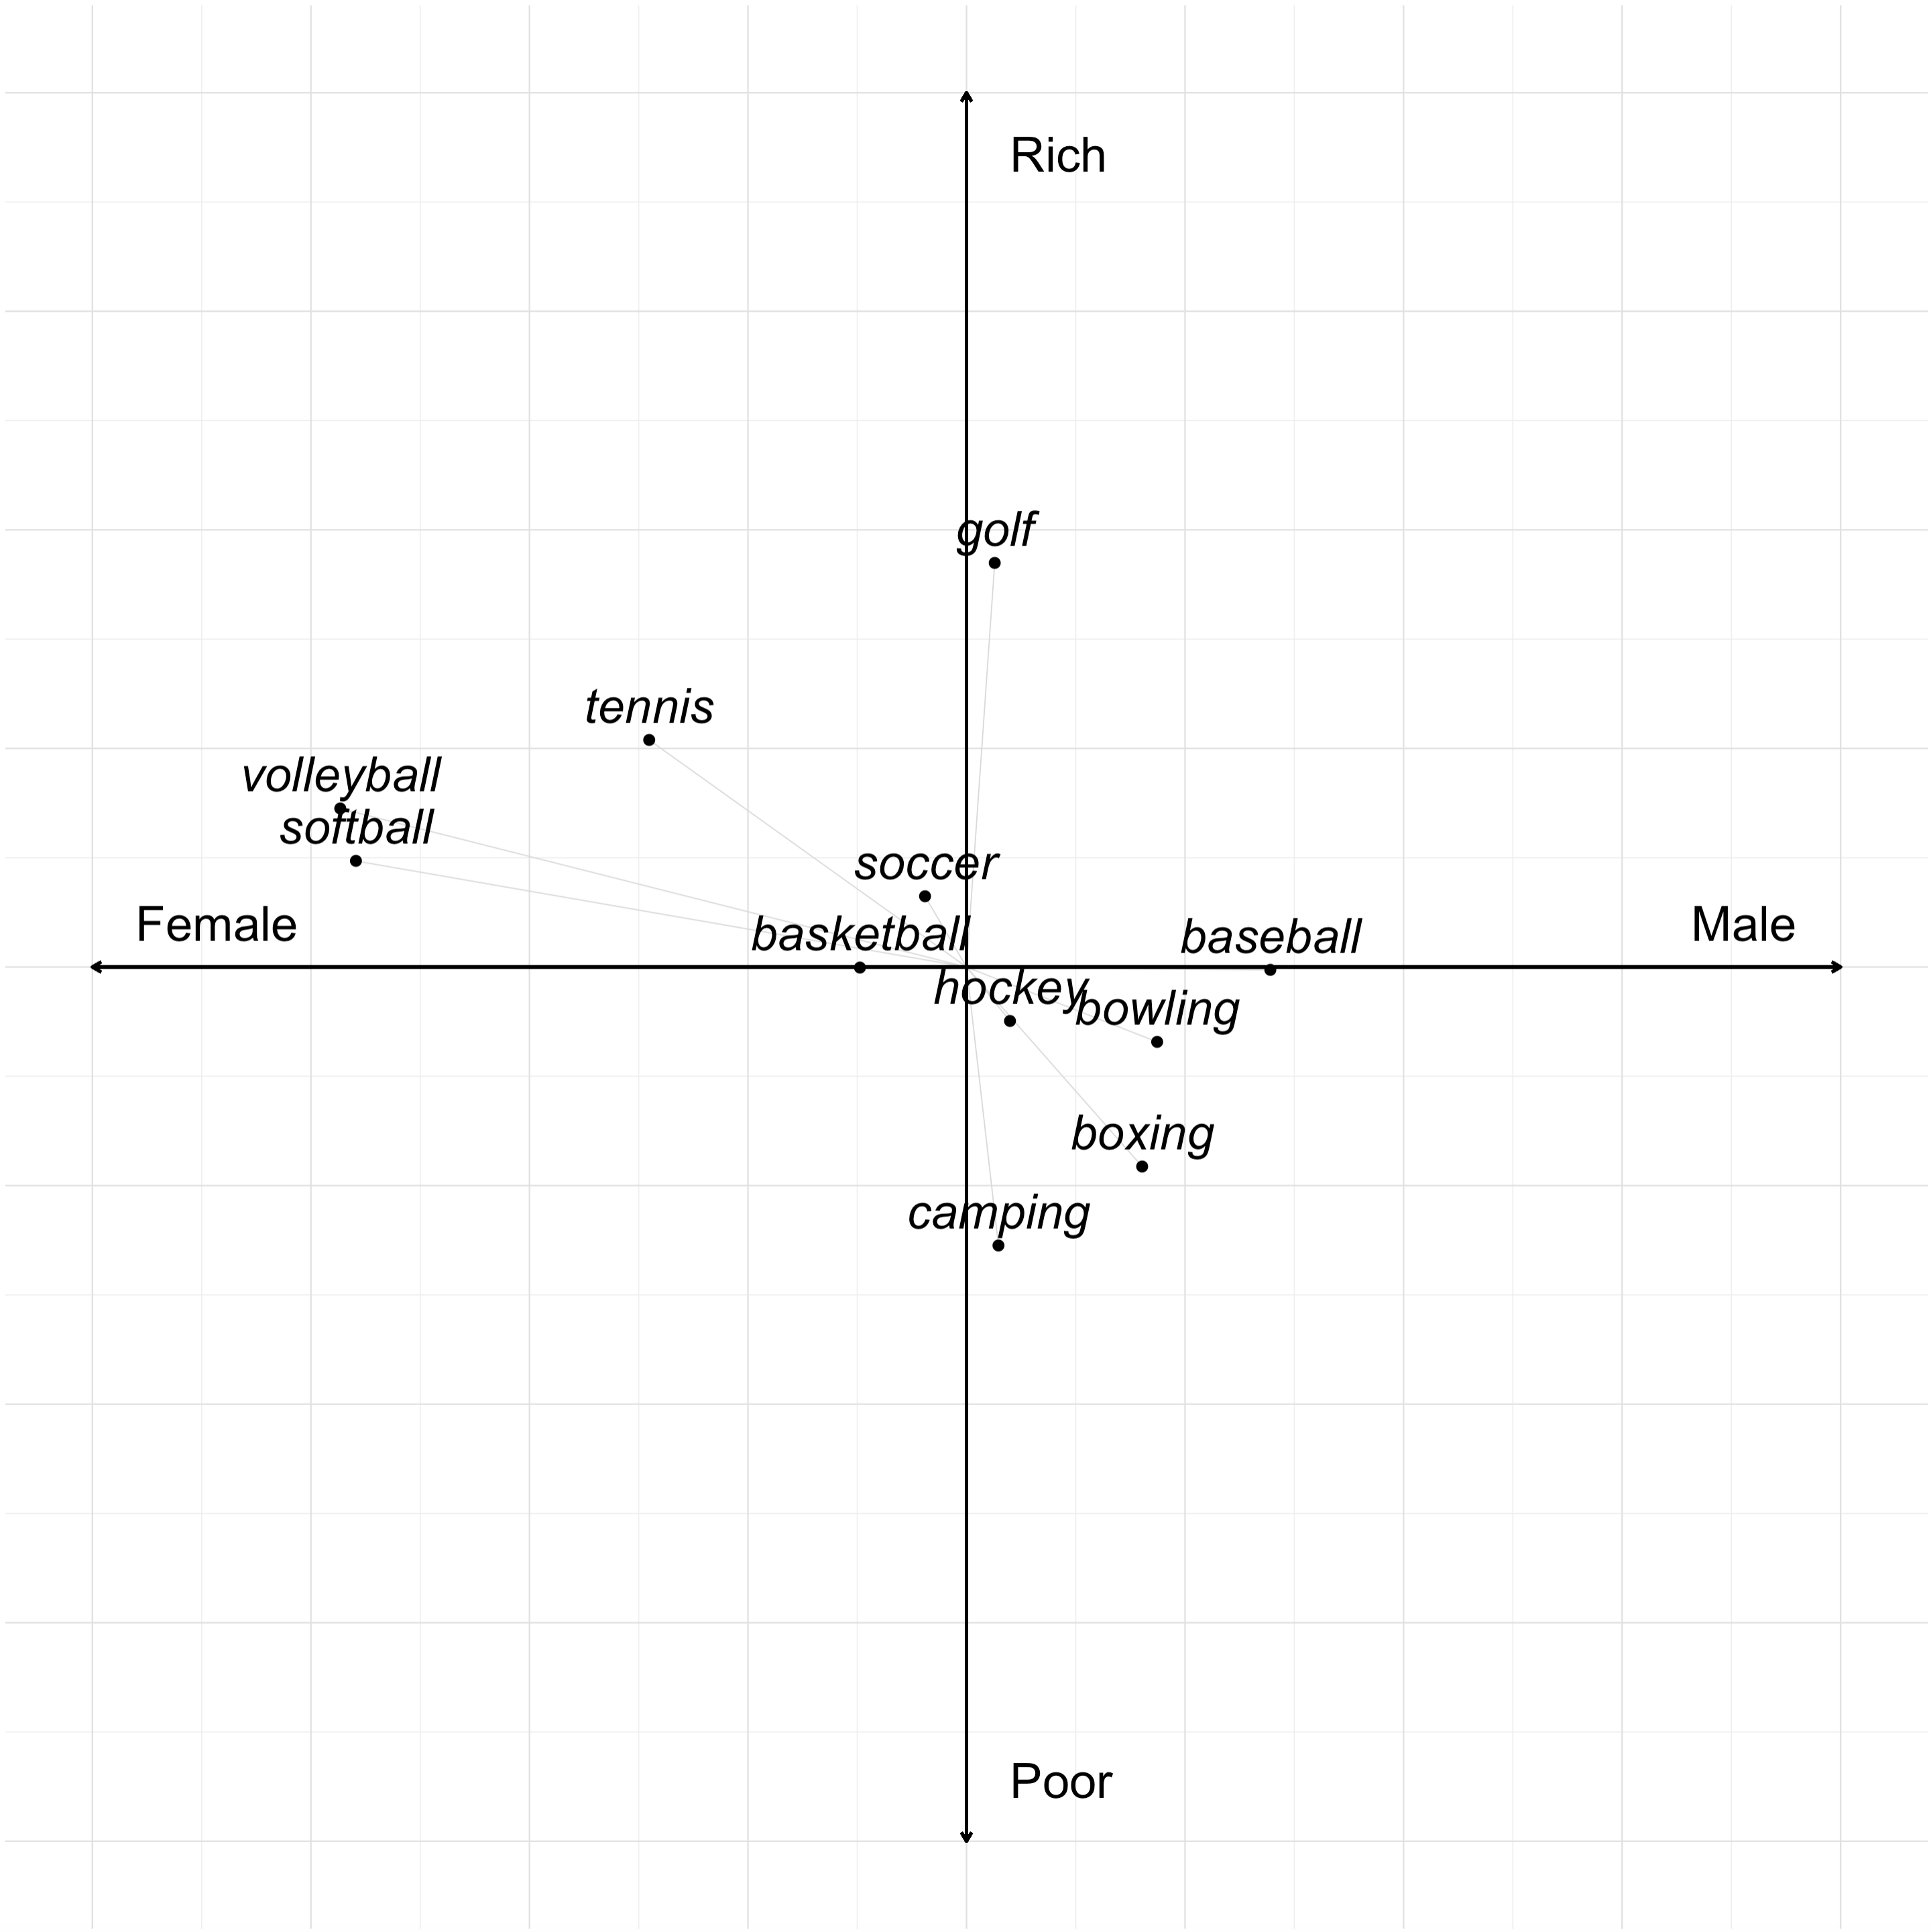
\includegraphics[width=.75\textwidth]{figures/media/kozlowski.png}
%   \caption{\label{fig:kozlowski}Semantische Projektion der Wortvektoren unterschiedlicher Sportarten auf zwei ‚kulturelle Dimensionen` (eigene Visualisierung von \emph{Figure} 2c aus \citealt[913]{kozlowskiGeometryCultureAnalyzing2019}).}

% 3 Methodik

% alt
Zum Durchbruch verhalfen Word Embeddings die von Mikolov et al. \autocite*{mikolovEfficientEstimationWord2013} bei Google entwickelten \emph{Word2Vec}-Algorithmen, mit denen die Ermittlung der Vektoren effizient und für große Datenmengen mit überschaubarem Hardware-Bedarf möglich wurde. Dabei wird ein neuronales Netz verwendet, mit dessen Hilfe Embeddings mit üblicherweise zwischen 200 und 600 Dimensionen berechnet werden können. Die Anzahl der Dimensionen liegt hier also deutlich unter der des oben zu Zwecken der Illustration skizzierten Beispiels, das die gesamte Type-Anzahl des Korpus als Dimensionen erfordern würde. Die Kehrseite dieses effizienteren Verfahrens ist, dass die einzelnen Werte der Dimensionen nicht unmittelbar interpretierbar sind. Sie stellen nun statt konkreten \emph{latente} semantische Features dar. Eine einzelne Dimension kann also etwas über das Kollokationsverhalten mit einer ganzen (unbekannten) Reihe anderer Wörter aussagen. Die Funktionsweise des neuronalen Netzes im Fall von \emph{Word2Vec} \autocite{mikolovEfficientEstimationWord2013} soll im Folgenden skizziert werden \autocite[siehe ausführlich][]{rongWord2vecParameterLearning2016}. Zunächst ist zwischen zwei Varianten des Algorithmus zu unterscheiden: \emph{Continuous Bag of Words} (CBOW) und \emph{Continuous Skip-gram} (Skip-Gram). Für beide Algorithmen wird das Korpus zunächst tokenisiert und in Sätze gegliedert. Im Anschluss erfolgt ein Training des neuronalen Netzes, indem es Vorhersagen über die Wörter im Satz -- in Abhängigkeit der sie umgebenden Wörter -- treffen muss. Während das Training neuronaler Netze in der Regel ein Trainingsdatenset voraussetzt, in dem die zu lernenden Features bereits (oftmals händisch) annotiert sind, nutzen Word-Embedding-Algorithmen das Korpus selbst als Trainingsgrundlage. Sie maskieren einzelne Wörter und sagen sie in Abhängigkeit anderer sie umgebender Wörter voraus -- kennen dabei ja aber stets die richtige Antwort und können so den Erfolg ihrer Vorhersage bewerten. Im Fall von CBOW wird ein Wort des Satzes maskiert und das Netz muss auf Basis des Kotextes (ein festzulegender Wert von per Default zwei Wörtern zur Linken und Rechten des Fokus-Wortes) vorhersagen, um welches Wort es sich handelt. Bei \emph{SkipGram} wird umgekehrt ein Wort vorgegeben und die Vorhersage erfolgt zum maskierten Kontext. Wesentliche Parameter für den Algorithmus sind die Anzahl der Dimensionen, die Variante (CBOW oder \emph{SkipGram}) und das Kontextfenster. Die Architektur des verwendeten neuronalen Netzes (siehe \figref{fig:cbow-architektur}) umfasst eine Eingabeschicht (\emph{input layer}), eine interne Repräsentation (\emph{projection layer}) sowie eine Ausgabeschicht (\emph{output layer}). Alle \emph{layer} entsprechen Vektoren einer bestimmten Länge und beinhalten Zahlenwerte. \emph{In}- und \emph{output layer} haben die Länge des Korpusvokabulars, während die Länge des \emph{projection layers} der festzulegenden Dimensionsanzahl entspricht.

\begin{figure}[t]
  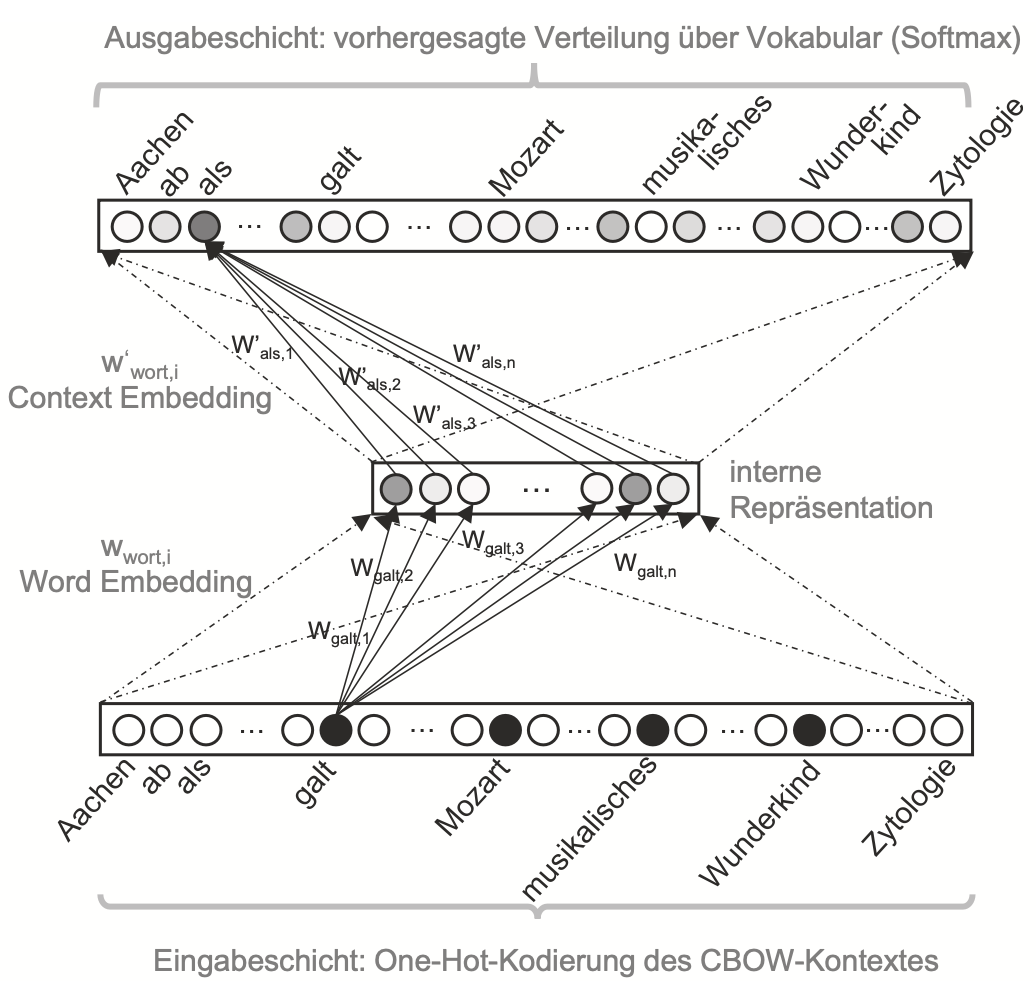
\includegraphics[width=\textwidth]{figures/media/image13.png}
  \caption{\label{fig:cbow-architektur}Schematische Darstellung der CBOW-Architektur für die Vorhersage von \emph{als} im Satz \emph{Mozart galt als musikalisches Wunderkind} (Abbildung 5.11 aus \citealt[221]{biemannWissensrohstoffTextEinfuehrung2022}).}
\end{figure}

~\figref{fig:cbow-architektur} zeigt eine schematische Darstellung für die CBOW-Variante des Algorithmus. Im unteren \emph{input layer} ist ausschnittsweise ein Vektor der Länge des Korpusvokabulars dargestellt, in dem die vier Kontextwörter \emph{galt}, \emph{Mozart}, \emph{musikalisch} und \emph{Wunderkind} markiert sind. Genau genommen verbergen sich dahinter vier Vektoren, jeweils in der Länge des Korpusvokabulars, die an jeder Stelle des Vokabulars eine 0 aufweisen, außer an der Stelle des jeweiligen Kontext-Wortes, das mit 1 markiert ist (sogenannte \emph{One-Hot}-Vektoren). Es finden im Anschluss in zwei Schritten Matrix-Multiplikationen statt: Zunächst wird jeder der vier \emph{One-Hot}-Vektoren mit \emph{n} zufällig initialisierten Werten, den sogenannten Gewichten, multipliziert und das arithmetische Mittel dieser vier Matrix-Multiplikationen (die ‚latente` oder ‚interne Repräsentation`) vom \emph{projection layer} in Richtung \emph{output layer} weitergegeben. Es findet nun erneut eine Matrix-Multiplikation mit zufällig initialisierten Werten statt. Dieses Mal entspricht die Anzahl der Gewichte jedoch der Größe des Vokabulars, d.\,h. der Anzahl der Korpus-Types. Das Ergebnis der Multiplikation sowie der nachfolgenden Anwendung der \emph{softmax}-Funktion\footnote{Mithilfe der \emph{softmax}-Funktion können die Werte von Vektoren in eine Wahrscheinlichhkeitsverteilung überführt werden.} findet sich im \emph{output layer}. Es handelt sich um einen Vektor der Länge des Vokabulars, wobei jeder Wert der Wahrscheinlichkeit des jeweiligen Wortes des Vokabulars in Abhängigkeit der Kontext-Wörter \emph{Mozart}, \emph{galt}, \emph{musikalisches} und \emph{Wunderkind} entspricht (das sogenannte \emph{context embedding}). Durch die dunkle Färbung der Vektordimension zu \emph{als} zeigt die Grafik an, dass das Training bereits fortgeschritten ist und das richtige Wort vorhergesagt wird. Der Ausgabevektor wird sodann mit dem Eingabevektor (Zielwort = 1, andere Wörter = 0) abgeglichen und die gemessene Differenz zwischen beiden zur Adjustierung der Gewichte genutzt (\emph{back propagation}). Während die \emph{context embeddings} i.d.R. nicht weiter genutzt werden,\footnote{Siehe aber z.\,B. Fankhauser \& Kupietz \autocite*{fankhauserCountBasedPredictiveLanguage2022}, die mit ihrer Hilfe Kollokationen \emph{prediction-} statt \emph{count-based} berechnen.} finden sich die eigentlichen \emph{n}-dimensionalen Word Embeddings in den Gewichten zwischen \emph{input} und \emph{projection layer}.

\hspace{-1mm} Zu beachten bei der Berechnung bzw. der Interpretation von Word-Embedding-Modellen (WEM) ist, dass ein WEM immer nur in sich schlüssig ist und die Embeddings eines Modells nicht mit denen anderer, unabhängig trainierter, Modelle verglichen werden können. Dies liegt in den Zufallskomponenten begründet, die beim Training des neuronalen Netzes wirksam sind. Man spricht bei diesen Algorithmen von nicht-deterministischen Algorithmen. Im Gegensatz zu ihren deterministischen Äquivalenten liefern sie auch bei gleicher Datengrundlage und gleichen Parametern keine identischen Ergebnisse. Es ist außerdem wichtig, auf eine möglichst große Datengrundlage und mithin eine möglichst große Anzahl an Kotexten für jedes Wort zurückgreifen zu können, um Zufallseinflüsse zu mindern.

% neu

% Zum Durchbruch verhalfen Word Embeddings die von Mikolov et al. \autocite*{mikolovEfficientEstimationWord2013} bei Google entwickelten \emph{Word2Vec}-Algorithmen, mit denen die Ermittlung der Vektoren effizient und für große Datenmengen mit überschaubarem Hardware-Bedarf möglich wurde. Dabei wird ein neuronales Netz verwendet, mit dessen Hilfe Embeddings mit üblicherweise zwischen 200 und 600 Dimensionen berechnet werden können. Die Anzahl der Dimensionen liegt hier also deutlich unter der des oben zu Zwecken der Illustration skizzierten Beispiels, das die gesamte Type-Anzahl des Korpus als Dimensionen erfordern würde. Die Kehrseite dieses effizienteren Verfahrens ist, dass die einzelnen Werte der Dimensionen nicht unmittelbar interpretierbar sind. Sie stellen nun statt konkreten \emph{latente} semantische Features dar. Eine einzelne Dimension kann also etwas über das Kollokationsverhalten mit einer ganzen (unbekannten) Reihe anderer Wörter aussagen. Die Funktionsweise des neuronalen Netzes im Fall von \emph{Word2Vec} \autocite{mikolovEfficientEstimationWord2013} soll im Folgenden skizziert werden \autocite[siehe ausführlich][]{rongWord2vecParameterLearning2016}. Zunächst ist zwischen zwei Varianten des Algorithmus zu unterscheiden: \emph{Continuous Bag of Words} (CBOW) und \emph{Continuous Skip-gram} (Skip-Gram). Für beide Algorithmen wird das Korpus zunächst tokenisiert und in Sätze gegliedert. Im Anschluss erfolgt ein Training des neuronalen Netzes, indem es Vorhersagen über die Wörter im Satz -- in Abhängigkeit der sie umgebenden Wörter -- treffen muss. Während das Training neuronaler Netze in der Regel ein Trainingsdatenset voraussetzt, in dem die zu lernenden Features bereits (oftmals händisch) annotiert sind, nutzen Word-Embedding-Algorithmen das Korpus selbst als Trainingsgrundlage. Sie maskieren einzelne Wörter und sagen sie in Abhängigkeit anderer sie umgebender Wörter voraus -- kennen dabei ja aber stets die richtige Antwort und können so den Erfolg ihrer Vorhersage bewerten. Im Fall von CBOW wird ein Wort des Satzes maskiert und das Netz muss auf Basis des Kotextes (ein festzulegender Wert von per Default fünf Wörtern zur Linken und Rechten des Fokus-Wortes) vorhersagen, um welches Wort es sich handelt. Bei \emph{SkipGram} wird umgekehrt ein Wort vorgegeben und die Vorhersage erfolgt zum maskierten Kontext. Wesentliche Parameter für den Algorithmus sind die Anzahl der Dimensionen, die Variante (CBOW oder \emph{SkipGram}) und das Kontextfenster. Die Architektur des verwendeten neuronalen Netzes (siehe \figref{fig:cbow-architektur}) umfasst eine Eingabeschicht (\emph{input layer}), eine interne Repräsentation (\emph{projection layer}) sowie eine Ausgabeschicht (\emph{output layer}). Alle \emph{layer} entsprechen Vektoren einer bestimmten Länge und beinhalten Zahlenwerte. \emph{In}- und \emph{output layer} haben die Länge des Korpusvokabulars, während die Länge des \emph{projection layers} der festzulegenden Dimensionsanzahl entspricht.
%
% \begin{figure}[t]
%   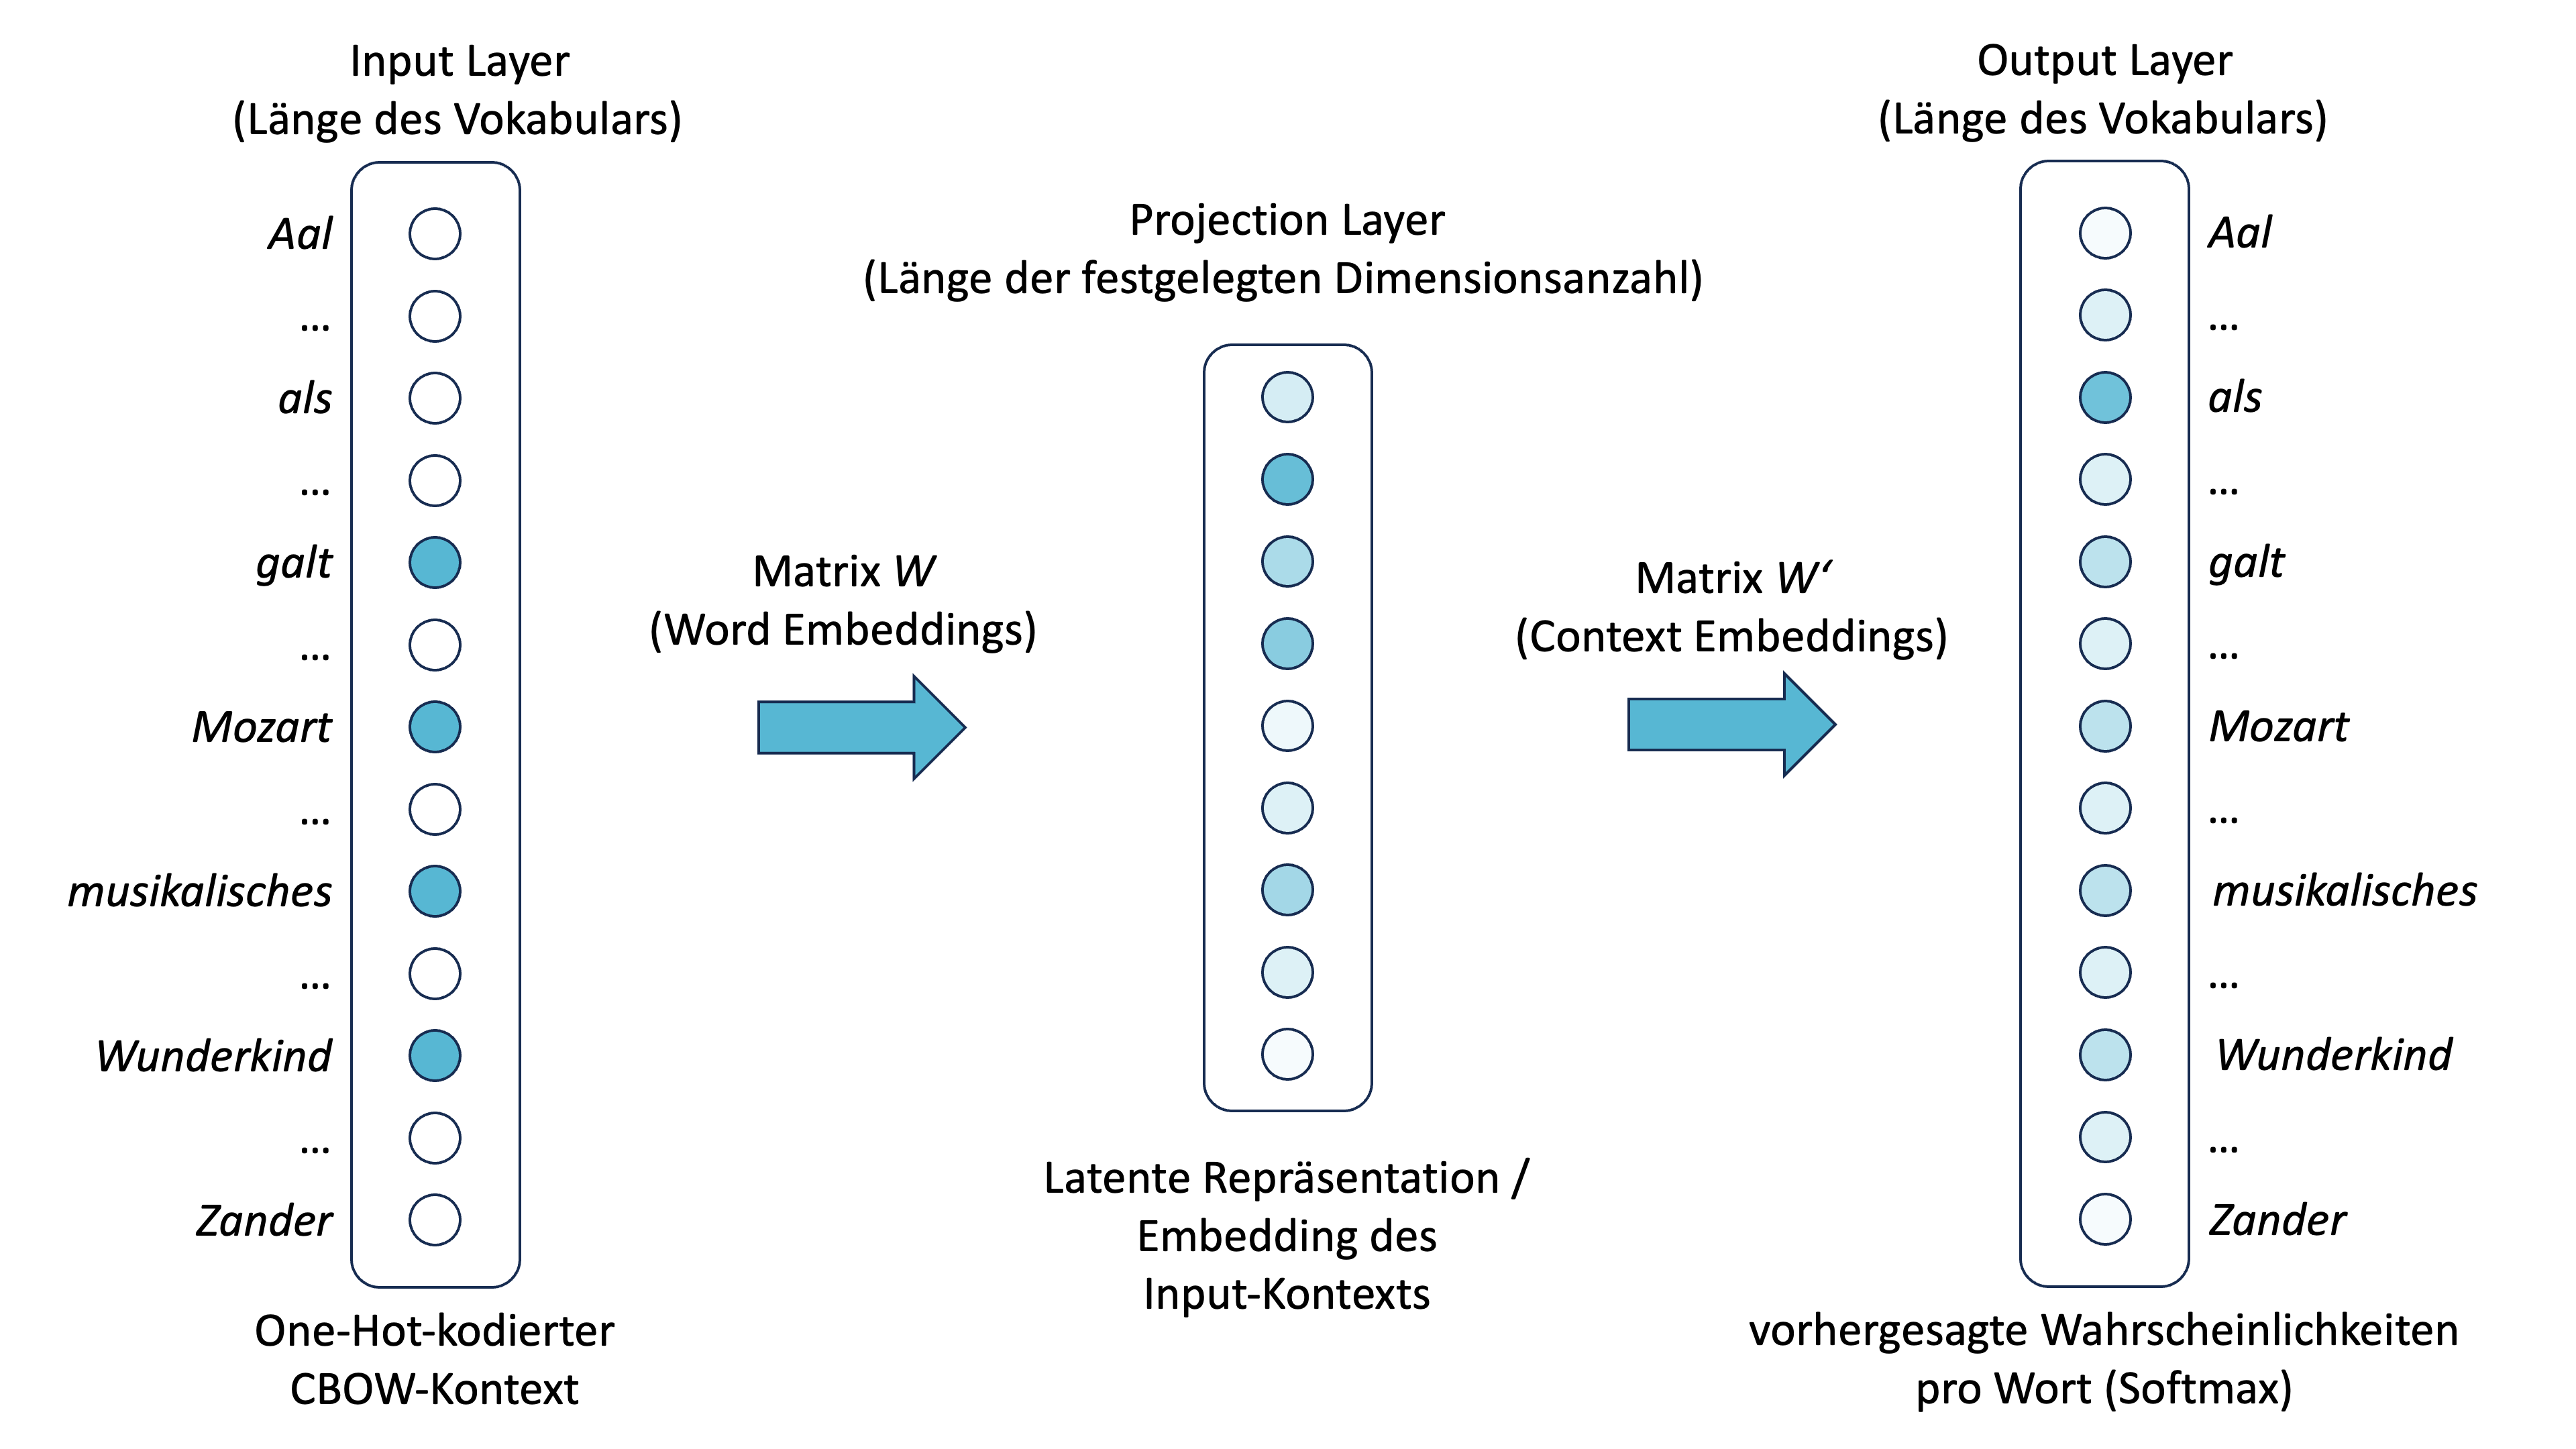
\includegraphics[width=\textwidth]{figures/media/grafik_cbow.png}
%   \caption{\label{fig:cbow-architektur}Schematische Darstellung der CBOW-Architektur für die Vorhersage von \emph{als} im Satz \emph{Mozart galt als musikalisches Wunderkind} (Adaption von Abbildung 5.11 aus \citealt[221]{biemannWissensrohstoffTextEinfuehrung2022}).}
% \end{figure}
%
% ~\figref{fig:cbow-architektur} zeigt eine schematische Darstellung für die CBOW-Variante des Algorithmus. Im unteren \emph{input layer} ist ausschnittsweise ein Vektor der Länge des Korpusvokabulars dargestellt, in dem die vier Kontextwörter \emph{galt}, \emph{Mozart}, \emph{musikalisch} und \emph{Wunderkind} markiert sind. Genau genommen verbergen sich dahinter vier Vektoren, jeweils in der Länge des Korpusvokabulars, die an jeder Stelle des Vokabulars eine 0 aufweisen, außer an der Stelle des jeweiligen Kontext-Wortes, das mit 1 markiert ist (sogenannte \emph{One-Hot}-Vektoren). Es finden im Anschluss in zwei Schritten Matrix-Multiplikationen (\emph{W} und \emph{W'}) statt: Zunächst wird jeder der vier \emph{One-Hot}-Vektoren mit \emph{n} zufällig initialisierten Werten, den sogenannten Gewichten, multipliziert und das arithmetische Mittel dieser vier Matrix-Multiplikationen (die ‚latente` oder ‚interne Repräsentation`) vom \emph{projection layer} in Richtung \emph{output layer} weitergegeben. Es findet nun erneut eine Matrix-Multiplikation mit zufällig initialisierten Werten statt. Dieses Mal entspricht die Anzahl der Gewichte jedoch der Größe des Vokabulars, d.\,h. der Anzahl der Korpus-Types. Das Ergebnis der Multiplikation sowie der nachfolgenden Anwendung der \emph{softmax}-Funktion\footnote{Mithilfe der \emph{softmax}-Funktion können die Werte von Vektoren in eine Wahrscheinlichhkeitsverteilung überführt werden.} findet sich im \emph{output layer}. Es handelt sich um einen Vektor der Länge des Vokabulars, wobei jeder Wert der Wahrscheinlichkeit des jeweiligen Wortes des Vokabulars in Abhängigkeit der Kontext-Wörter \emph{Mozart}, \emph{galt}, \emph{musikalisches} und \emph{Wunderkind} entspricht. Durch die dunkle Färbung der Vektordimension zu \emph{als} zeigt die Grafik an, dass das Training bereits fortgeschritten ist und das richtige Wort vorhergesagt wird. Der Ausgabevektor wird sodann mit dem Eingabevektor (Zielwort = 1, andere Wörter = 0) abgeglichen und die gemessene Differenz zwischen beiden zur Adjustierung der Gewichte genutzt (\emph{back propagation}). Während die \emph{context embeddings} i.d.R. nicht weiter genutzt werden,\footnote{Siehe aber z.\,B. Fankhauser \& Kupietz \autocite*{fankhauserCountBasedPredictiveLanguage2022}, die mit ihrer Hilfe Kollokationen \emph{prediction-} statt \emph{count-based} berechnen.} finden sich die eigentlichen \emph{n}-dimensionalen Word Embeddings in den Gewichten zwischen \emph{input} und \emph{projection layer}, d.h. in Matrix \emph{W}.
%
% \hspace{-1mm} Zu beachten bei der Berechnung bzw. der Interpretation von Word-Embedding-Modellen (WEM) ist, dass ein WEM immer nur in sich schlüssig ist und die Embeddings eines Modells nicht mit denen anderer, unabhängig trainierter, Modelle verglichen werden können. Dies liegt in den Zufallskomponenten begründet, die beim Training des neuronalen Netzes wirksam sind. Man spricht bei diesen Algorithmen von nicht-deterministischen Algorithmen. Im Gegensatz zu ihren deterministischen Äquivalenten liefern sie auch bei gleicher Datengrundlage und gleichen Parametern keine identischen Ergebnisse. Es ist außerdem wichtig, auf eine möglichst große Datengrundlage und mithin eine möglichst große Anzahl an Kotexten für jedes Wort zurückgreifen zu können, um Zufallseinflüsse zu mindern.
6]).}
% alt
%   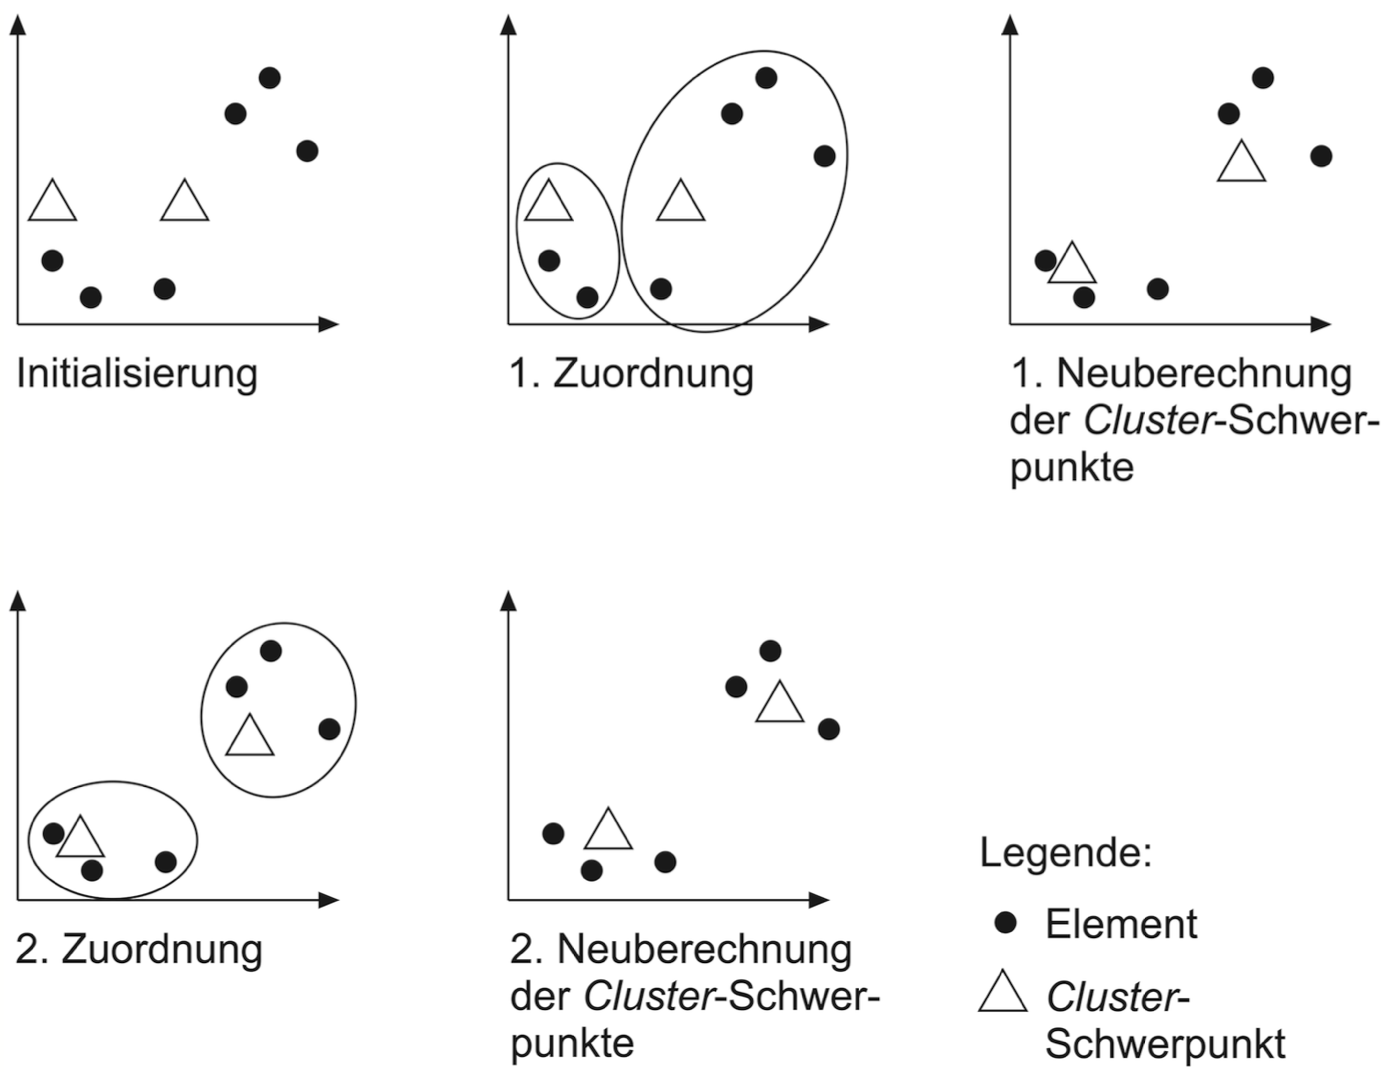
\includegraphics[width=\textwidth]{figures/media/image14.png}
%   \caption{\label{fig:kmeans-beispiel-k2}Illustration des \emph{k-Means}-Algorithmus bei \emph{k} = 2 und sechs Vektoren (Abbildung 6.5 aus \citealt[270]{biemannWissensrohstoffTextEinfuehrung2022}).}
% % neu
%   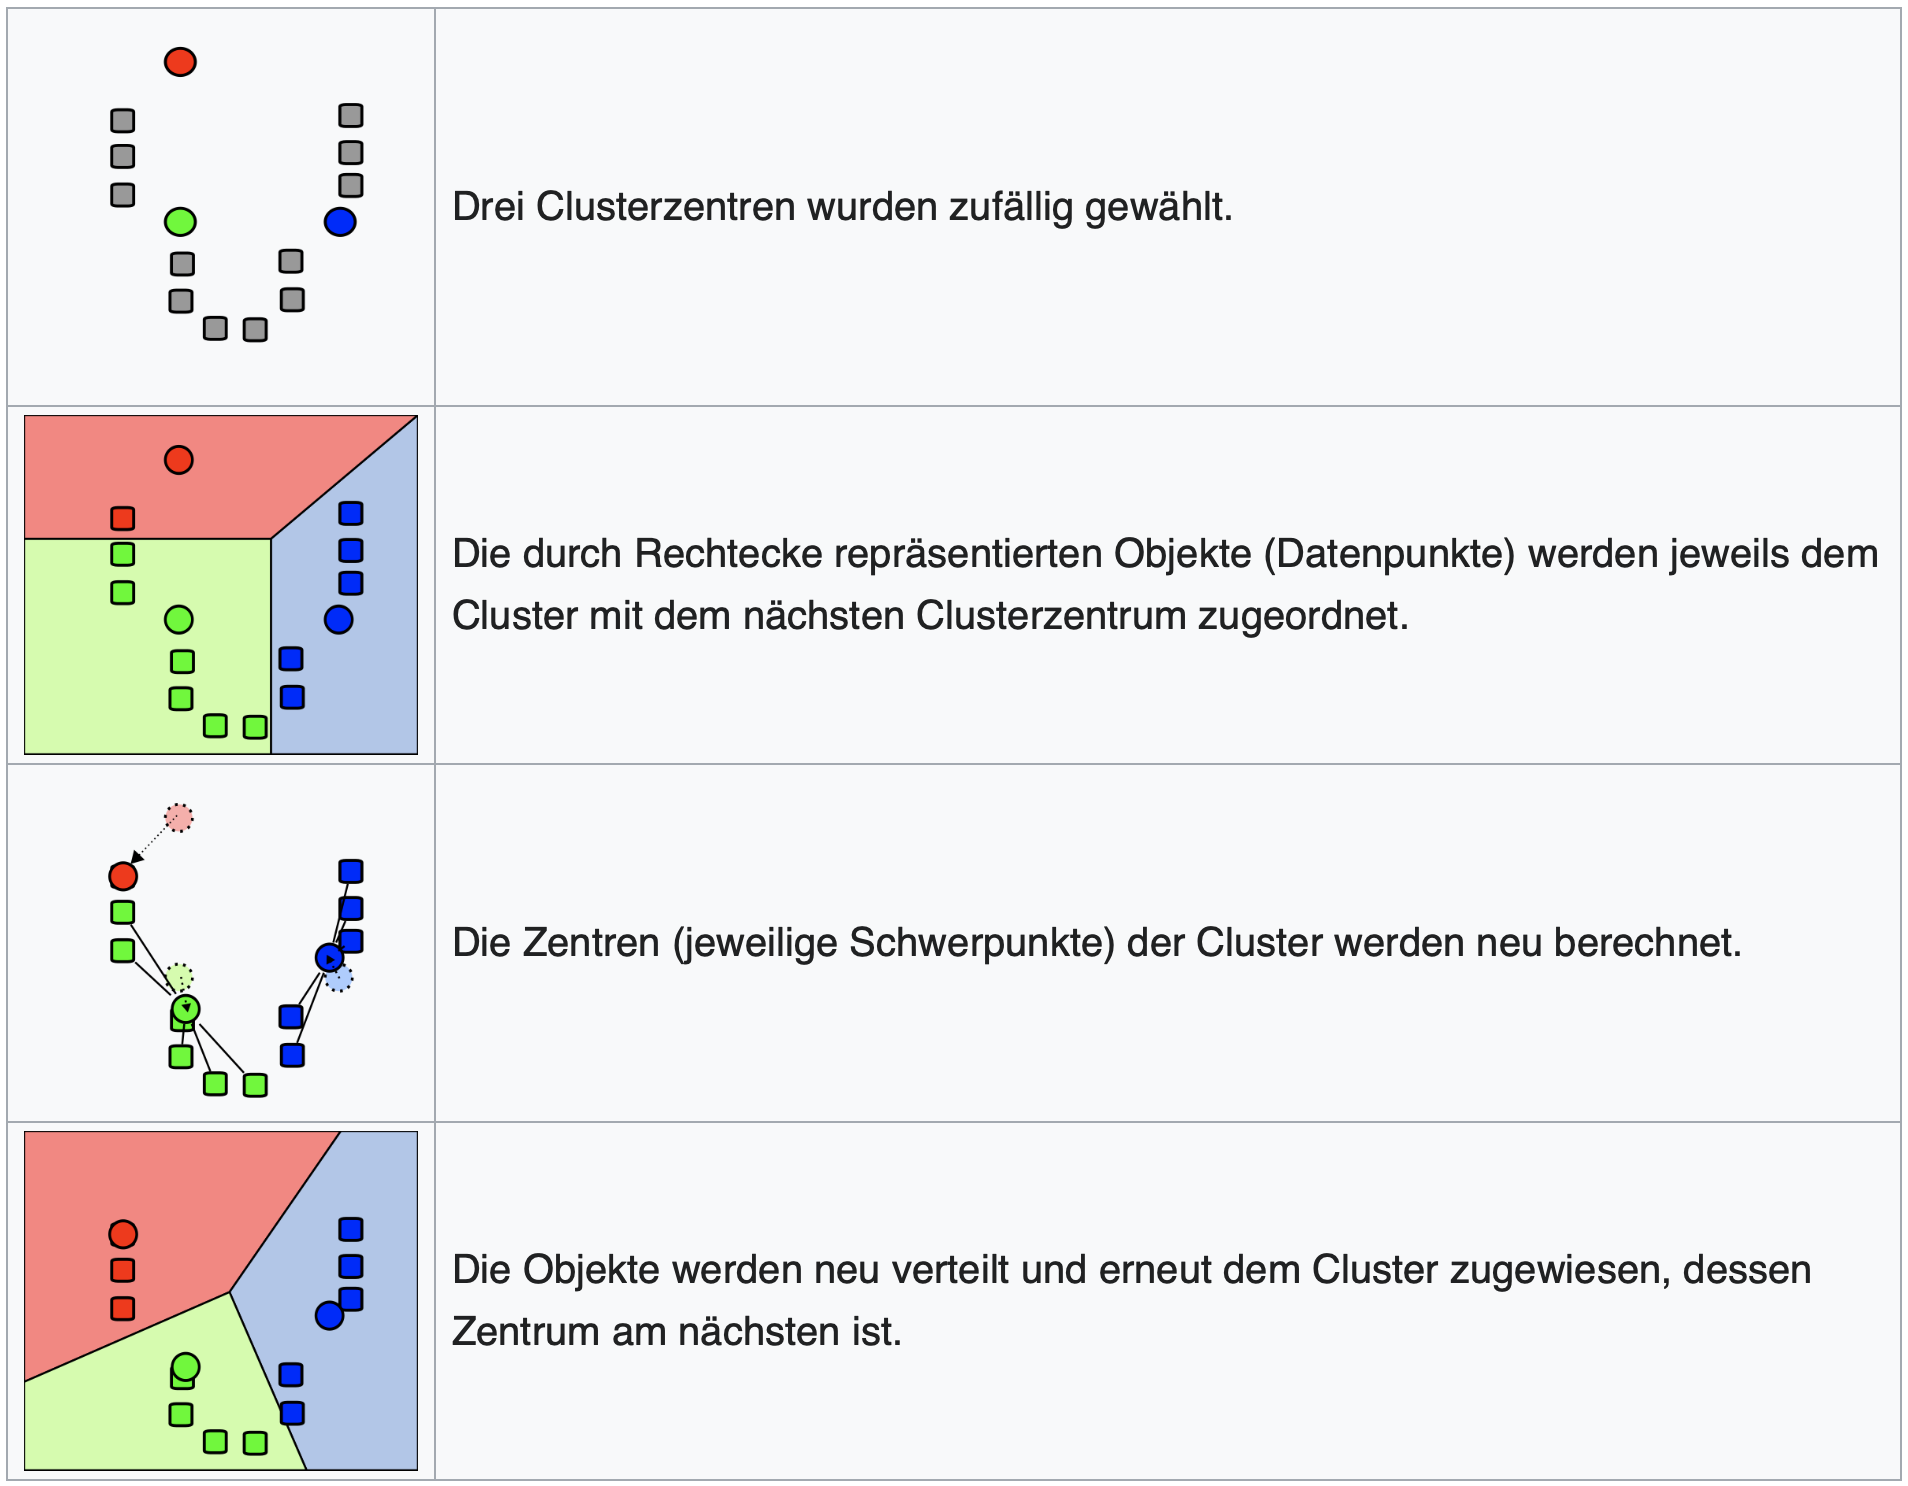
\includegraphics[width=\textwidth]{figures/media/kmeans.png}
%   \caption{\label{fig:kmeans-beispiel-k2}Illustration des \emph{k-Means}-Algorithmus bei \emph{k} = 3 und zwölf Vektoren (Urheber der Grafiken: weston.pace, CC BY-SA 3.0, \url{https://de.wikipedia.org/wiki/K-Means-Algorithmus} [31.01.202

% alt
Durch die Zufallskomponente bei der Initialisierung handelt es sich auch bei \emph{k-Means} um einen nicht-deterministischen Algorithmus, sodass die Zuordnungen der Wörter zu Clustern im Verlauf mehrerer Ausführungen variieren kann. Zu beachten ist darüber hinaus, dass wie Grand et al. \autocite*{grandSemanticProjectionRecovers2022} hervorheben, Nähe von Word Embeddings im Vektorraum immer auf einer globalen semantischen Ähnlichkeit beruht, die sich eigentlich in die Positionierung entlang einer Vielzahl semantischer Dimensionen aufspalten ließe. Je nachdem, was als \emph{tertium comparationis} gewählt ist, können also unterschiedliche Nachbarschaften von Wörtern entstehen. So weisen, wie in \figref{fig:tiere-embeddings-semantik} gezeigt, die Wörter \emph{dolphin} und \emph{tiger} eine mehr oder weniger große Distanz auf, je nachdem, auf welche semantische Dimension des Vektorraums man sie projiziert.

\begin{figure}
  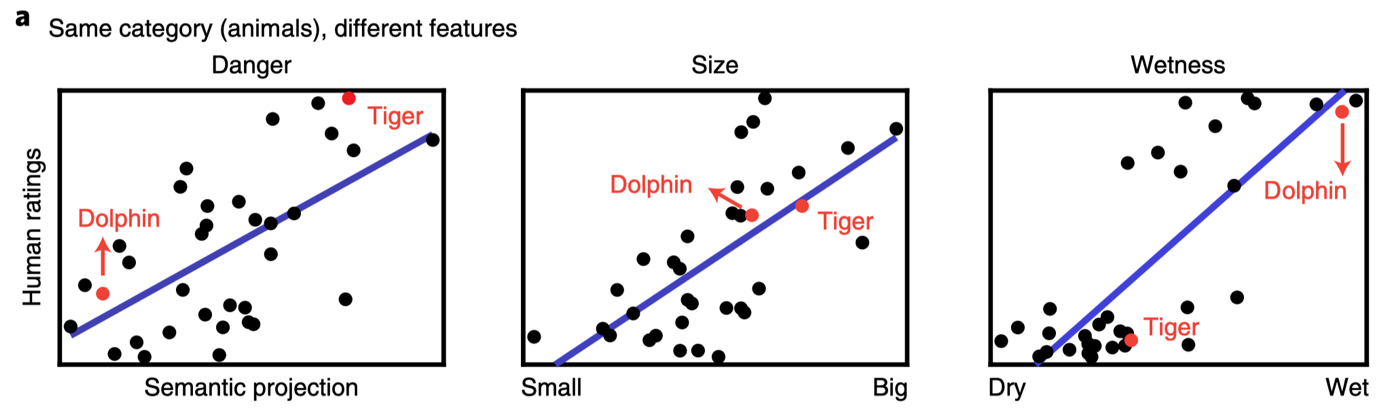
\includegraphics[width=\textwidth]{figures/media/image15.png}
  \caption{\label{fig:tiere-embeddings-semantik}Korrelation zwischen der Projektion der Word Embeddings unterschiedlicher Tiere auf unterschiedliche semantische Achsen und menschlichen Bewertungen (\emph{Figure 2a} aus \citealt{grandSemanticProjectionRecovers2022}).}
\end{figure}
% neu
Durch die Zufallskomponente bei der Initialisierung handelt es sich auch bei \emph{k-Means} um einen nicht-deterministischen Algorithmus, sodass die Zuordnungen der Wörter zu Clustern im Verlauf mehrerer Ausführungen variieren kann. Zu beachten ist darüber hinaus, dass wie Grand et al. \autocite*{grandSemanticProjectionRecovers2022} hervorheben, Nähe von Word Embeddings im Vektorraum immer auf einer globalen semantischen Ähnlichkeit beruht, die sich eigentlich in die Positionierung entlang einer Vielzahl semantischer Dimensionen aufspalten ließe. Je nachdem, was als \emph{tertium comparationis} gewählt ist, können also unterschiedliche Nachbarschaften von Wörtern entstehen. So weisen die Wörter \emph{dolphin} und \emph{tiger} eine geringe Distanz auf, wenn man sie auf die Dimension \emph{size} projiziert; jedoch eine große Distanz bei Projektion auf die Dimension \emph{danger} (siehe \emph{Figure 2a} in \citealt{grandSemanticProjectionRecovers2022}).
